% $Header: /u/gcmpack/manual/s_autodiff/text/doc_ad_2.tex,v 1.19 2005/08/02 22:26:58 heimbach Exp $
% $Name:  $

Author: Patrick Heimbach

{\sf Automatic differentiation} (AD), also referred to as algorithmic
(or, more loosely, computational) differentiation, involves 
automatically deriving code to calculate
partial derivatives from an existing fully non-linear prognostic code.
(see \cite{gri:00}).
A software tool is used that parses and transforms source files 
according to a set of linguistic and mathematical rules. 
AD tools are like source-to-source translators in that
they parse a program code as input and produce a new program code 
as output.
However, unlike a pure source-to-source translation, the output program
represents a new algorithm, such as the evaluation of the
Jacobian, the Hessian, or higher derivative operators.
In principle, a variety of derived algorithms
can be generated automatically in this way.

The MITGCM has been adapted for use with the
Tangent linear and Adjoint Model Compiler (TAMC) and its successor TAF
(Transformation of Algorithms in Fortran), developed
by Ralf Giering (\cite{gie-kam:98}, \cite{gie:99,gie:00}).
The first application of the adjoint of the MITGCM for sensitivity
studies has been published by \cite{maro-eta:99}.
\cite{sta-eta:97,sta-eta:01} use the MITGCM and its adjoint
for ocean state estimation studies.
In the following we shall refer to TAMC and TAF synonymously,
except were explicitly stated otherwise.

TAMC exploits the chain rule for computing the first
derivative of a function with
respect to a set of input variables. 
Treating a given forward code as a composition of operations --
each line representing a compositional element, the chain rule is
rigorously applied to the code, line by line. The resulting 
tangent linear or adjoint code,
then, may be thought of as the composition in 
forward or reverse order, respectively, of the
Jacobian matrices of the forward code's compositional elements.

%**********************************************************************
\section{Some basic algebra}
\label{sec_ad_algebra}
\begin{rawhtml}
<!-- CMIREDIR:sec_ad_algebra: -->
\end{rawhtml}
%**********************************************************************

Let $ \cal{M} $ be a general nonlinear, model, i.e. a
mapping from the $m$-dimensional space 
$U \subset I\!\!R^m$ of input variables 
$\vec{u}=(u_1,\ldots,u_m)$
(model parameters, initial conditions, boundary conditions
such as forcing functions) to the $n$-dimensional space 
$V \subset I\!\!R^n$ of 
model output variable $\vec{v}=(v_1,\ldots,v_n)$ 
(model state, model diagnostics, objective function, ...) 
under consideration,
%
\begin{equation}
\begin{split}
{\cal M} \, : & \, U \,\, \longrightarrow \, V \\
~      & \, \vec{u} \,\, \longmapsto \, \vec{v} \, = \, 
{\cal M}(\vec{u}) 
\label{fulloperator}
\end{split}
\end{equation}
%
The vectors $ \vec{u} \in U $ and $ v \in V $ may be represented w.r.t.
some given basis vectors
$ {\rm span} (U) = \{ {\vec{e}_i} \}_{i = 1, \ldots , m} $ and
$ {\rm span} (V) = \{ {\vec{f}_j} \}_{j = 1, \ldots , n} $ as
\[
\vec{u} \, = \, \sum_{i=1}^{m} u_i \, {\vec{e}_i},
\qquad
\vec{v} \, = \, \sum_{j=1}^{n} v_j \, {\vec{f}_j}
\]

Two routes may be followed to determine the sensitivity of the 
output variable $\vec{v}$ to its input $\vec{u}$.

\subsection{Forward or direct sensitivity}
%
Consider a perturbation to the input variables $\delta \vec{u}$
(typically a single component 
$\delta \vec{u} = \delta u_{i} \, {\vec{e}_{i}}$).
Their effect on the output may be obtained via the linear
approximation of the model $ {\cal M}$ in terms of its Jacobian matrix
$ M $, evaluated in the point $u^{(0)}$ according to
%
\begin{equation}
\delta \vec{v} \, = \, M |_{\vec{u}^{(0)}} \, \delta \vec{u}
\label{tangent_linear}
\end{equation}
with resulting output perturbation $\delta \vec{v}$.
In components
$M_{j i} \, = \, \partial {\cal M}_{j} / \partial u_{i} $, 
it reads
%
\begin{equation}
\delta v_{j} \, = \, \sum_{i} 
\left. \frac{\partial {\cal M}_{j}}{\partial u_{i}} \right|_{u^{(0)}} \, 
\delta u_{i}
\label{jacobi_matrix}
\end{equation}
%
Eq. (\ref{tangent_linear}) is the {\sf tangent linear model (TLM)}.
In contrast to the full nonlinear model $ {\cal M} $, the operator
$ M $ is just a matrix
which can readily be used to find the forward sensitivity of $\vec{v}$ to 
perturbations in  $u$,
but if there are very many input variables $(\gg O(10^{6})$ for 
large-scale oceanographic application), it quickly becomes 
prohibitive to proceed directly as in (\ref{tangent_linear}),
if the impact of each component $ {\bf e_{i}} $ is to be assessed. 

\subsection{Reverse or adjoint sensitivity}
%
Let us consider the special case of a
scalar objective function ${\cal J}(\vec{v})$ of the model output (e.g. 
the total meridional heat transport, 
the total uptake of $CO_{2}$ in the Southern 
Ocean over a time interval,
or a measure of some model-to-data misfit)
%
\begin{eqnarray}
\begin{array}{cccccc}
{\cal J}  \, : &  U & 
\longrightarrow & V &   
\longrightarrow & I \!\! R \\
~       &  \vec{u} & \longmapsto     & \vec{v}={\cal M}(\vec{u}) & 
\longmapsto     & {\cal J}(\vec{u}) = {\cal J}({\cal M}(\vec{u}))
\end{array}
\label{compo}
\end{eqnarray}
%
The perturbation of $ {\cal J} $ around a fixed point $ {\cal J}_0 $,
\[
{\cal J} \, = \, {\cal J}_0 \, + \, \delta {\cal J}
\]
can be expressed in both bases of $ \vec{u} $ and $ \vec{v} $
w.r.t. their corresponding inner product 
$\left\langle \,\, , \,\, \right\rangle $ 
%
\begin{equation}
\begin{split}
{\cal J} & = \,
{\cal J} |_{\vec{u}^{(0)}} \, + \, 
\left\langle \, \nabla _{u}{\cal J}^T |_{\vec{u}^{(0)}} \, , \, \delta \vec{u} \, \right\rangle 
\, + \, O(\delta \vec{u}^2) \\
~ & = \,
{\cal J} |_{\vec{v}^{(0)}} \, + \, 
\left\langle \, \nabla _{v}{\cal J}^T |_{\vec{v}^{(0)}} \, , \, \delta \vec{v} \, \right\rangle
\, + \, O(\delta \vec{v}^2)
\end{split}
\label{deljidentity}
\end{equation}
%
(note, that the gradient $ \nabla f $ is a co-vector, therefore
its transpose is required in the above inner product).
Then, using the representation of 
$ \delta {\cal J} = 
\left\langle \, \nabla _{v}{\cal J}^T \, , \, \delta \vec{v} \, \right\rangle $,
the definition 
of an adjoint operator $ A^{\ast} $ of a given operator $ A $,
\[ 
\left\langle \, A^{\ast} \vec{x} \, , \, \vec{y} \, \right\rangle =
\left\langle \, \vec{x} \, , \,  A \vec{y} \, \right\rangle 
\]
which for finite-dimensional vector spaces is just the 
transpose of $ A $,
\[
A^{\ast} \, = \, A^T
\]
and from eq. (\ref{tangent_linear}), (\ref{deljidentity}),
we note that
(omitting $|$'s):
%
\begin{equation}
\delta {\cal J}
\, = \,
\left\langle \, \nabla _{v}{\cal J}^T \, , \, \delta \vec{v} \, \right\rangle
\, = \,
\left\langle \, \nabla _{v}{\cal J}^T \, , \, M \, \delta \vec{u} \, \right\rangle
\, = \, 
\left\langle \, M^T \, \nabla _{v}{\cal J}^T \, , \, 
\delta \vec{u} \, \right\rangle
\label{inner}
\end{equation}
%
With the identity (\ref{deljidentity}), we then find that
the gradient $ \nabla _{u}{\cal J} $ can be readily inferred by 
invoking the adjoint $ M^{\ast } $ of the tangent linear model $ M $
%
\begin{equation}
\begin{split}
\nabla _{u}{\cal J}^T |_{\vec{u}} & 
= \, M^T |_{\vec{u}} \cdot \nabla _{v}{\cal J}^T |_{\vec{v}}  \\
~ & = \, M^T |_{\vec{u}} \cdot \delta \vec{v}^{\ast} \\
~ & = \, \delta \vec{u}^{\ast}
\end{split}
\label{adjoint}
\end{equation}
%
Eq. (\ref{adjoint}) is the {\sf adjoint model (ADM)}, 
in which $M^T$ is the adjoint (here, the transpose) of the 
tangent linear operator $M$, $ \delta \vec{v}^{\ast} $ 
the adjoint variable of the model state $ \vec{v} $, and
$ \delta \vec{u}^{\ast} $ the adjoint variable of the control variable $ \vec{u} $.

The {\sf reverse} nature of the adjoint calculation can be readily 
seen as follows. 
Consider a model integration which consists of $ \Lambda $
consecutive operations
$ {\cal M}_{\Lambda} (  {\cal M}_{\Lambda-1} ( 
...... ( {\cal M}_{\lambda} (
......
( {\cal M}_{1} ( {\cal M}_{0}(\vec{u}) )))) $,
where the ${\cal M}$'s could be the elementary steps, i.e. single lines
in the code of the model, or successive time steps of the
model integration, 
starting at step 0 and moving up to step $\Lambda$, with intermediate
${\cal M}_{\lambda} (\vec{u}) = \vec{v}^{(\lambda+1)}$ and final 
${\cal M}_{\Lambda} (\vec{u}) = \vec{v}^{(\Lambda+1)} = \vec{v}$.
Let ${\cal J}$ be a cost function which explicitly depends on the
final state $\vec{v}$ only
(this restriction is for clarity reasons only).
%
${\cal J}(u)$ may be decomposed according to:
%
\begin{equation}
{\cal J}({\cal M}(\vec{u})) \, = \, 
{\cal J} ( {\cal M}_{\Lambda} (  {\cal M}_{\Lambda-1} ( 
...... ( {\cal M}_{\lambda} (
......
( {\cal M}_{1} ( {\cal M}_{0}(\vec{u}) )))))
\label{compos}
\end{equation}
%
Then, according to the chain rule, the forward calculation reads, 
in terms of the Jacobi matrices
(we've omitted the $ | $'s which, nevertheless are important
to the aspect of {\it tangent} linearity;
note also that by definition
$ \langle \, \nabla _{v}{\cal J}^T \, , \, \delta \vec{v} \, \rangle
= \nabla_v {\cal J} \cdot \delta \vec{v} $ )
%
\begin{equation}
\begin{split}
\nabla_v {\cal J} (M(\delta \vec{u})) & = \,
\nabla_v {\cal J} \cdot M_{\Lambda}
\cdot ...... \cdot M_{\lambda} \cdot ...... \cdot
M_{1} \cdot M_{0} \cdot \delta \vec{u} \\
~ & = \, \nabla_v {\cal J} \cdot \delta \vec{v} \\
\end{split}
\label{forward}
\end{equation}
%
whereas in reverse mode we have
%
\begin{equation}
\boxed{
\begin{split}
M^T ( \nabla_v {\cal J}^T) & = \,
M_{0}^T \cdot M_{1}^T
\cdot ...... \cdot M_{\lambda}^T \cdot ...... \cdot 
M_{\Lambda}^T \cdot \nabla_v {\cal J}^T \\
~ & = \, M_{0}^T \cdot M_{1}^T
\cdot ...... \cdot 
\nabla_{v^{(\lambda)}} {\cal J}^T \\
~ & = \, \nabla_u {\cal J}^T
\end{split}
}
\label{reverse}
\end{equation}
%
clearly expressing the reverse nature of the calculation.
Eq. (\ref{reverse}) is at the heart of automatic adjoint compilers.
If the intermediate steps $\lambda$ in 
eqn. (\ref{compos}) -- (\ref{reverse})
represent the model state (forward or adjoint) at each 
intermediate time step as noted above, then correspondingly,
$ M^T (\delta \vec{v}^{(\lambda) \, \ast}) = 
\delta \vec{v}^{(\lambda-1) \, \ast} $ for the adjoint variables.
It thus becomes evident that the adjoint calculation also
yields the adjoint of each model state component 
$ \vec{v}^{(\lambda)} $ at each intermediate step $ \lambda $, namely
%
\begin{equation}
\boxed{
\begin{split}
\nabla_{v^{(\lambda)}} {\cal J}^T |_{\vec{v}^{(\lambda)}}
& = \,
M_{\lambda}^T |_{\vec{v}^{(\lambda)}} \cdot ...... \cdot 
M_{\Lambda}^T |_{\vec{v}^{(\lambda)}} \cdot \delta \vec{v}^{\ast} \\
~ & = \, \delta \vec{v}^{(\lambda) \, \ast}
\end{split}
}
\end{equation}
%
in close analogy to eq. (\ref{adjoint})
We note in passing that that the $\delta \vec{v}^{(\lambda) \, \ast}$
are the Lagrange multipliers of the model equations which determine
$ \vec{v}^{(\lambda)}$.

In components, eq. (\ref{adjoint}) reads as follows.
Let
\[
\begin{array}{rclcrcl}
\delta \vec{u} & = &
\left( \delta u_1,\ldots, \delta u_m \right)^T , & \qquad &
\delta \vec{u}^{\ast} \,\, = \,\, \nabla_u {\cal J}^T & = &
\left( 
\frac{\partial {\cal J}}{\partial u_1},\ldots, 
\frac{\partial {\cal J}}{\partial u_m}
\right)^T \\
\delta \vec{v} & = &
\left( \delta v_1,\ldots, \delta u_n \right)^T , & \qquad &
\delta \vec{v}^{\ast} \,\, = \,\, \nabla_v {\cal J}^T & = &
\left( 
\frac{\partial {\cal J}}{\partial v_1},\ldots, 
\frac{\partial {\cal J}}{\partial v_n}
\right)^T \\
\end{array}
\]
denote the perturbations in $\vec{u}$ and $\vec{v}$, respectively,
and their adjoint variables;
further
\[
M \, = \, \left(
\begin{array}{ccc}
\frac{\partial {\cal M}_1}{\partial u_1} & \ldots &
\frac{\partial {\cal M}_1}{\partial u_m} \\
\vdots & ~ & \vdots \\
\frac{\partial {\cal M}_n}{\partial u_1} & \ldots &
\frac{\partial {\cal M}_n}{\partial u_m} \\
\end{array}
\right)
\]
is the Jacobi matrix of $ {\cal M} $ 
(an $ n \times m $ matrix)
such that $ \delta \vec{v} = M \cdot \delta \vec{u} $, or
\[
\delta v_{j} 
\, = \, \sum_{i=1}^m M_{ji} \, \delta u_{i}
\, = \, \sum_{i=1}^m \, \frac{\partial {\cal M}_{j}}{\partial u_{i}} 
\delta u_{i}
\]
%
Then eq. (\ref{adjoint}) takes the form
\[
\delta u_{i}^{\ast} 
\, = \, \sum_{j=1}^n M_{ji} \, \delta v_{j}^{\ast}
\, = \, \sum_{j=1}^n \, \frac{\partial {\cal M}_{j}}{\partial u_{i}} 
\delta v_{j}^{\ast}
\]
%
or
%
\[
\left(
\begin{array}{c}
\left. \frac{\partial}{\partial u_1} {\cal J} \right|_{\vec{u}^{(0)}} \\
\vdots \\
\left. \frac{\partial}{\partial u_m} {\cal J} \right|_{\vec{u}^{(0)}} \\
\end{array}
\right)
\, = \,
\left(
\begin{array}{ccc}
\left. \frac{\partial {\cal M}_1}{\partial u_1} \right|_{\vec{u}^{(0)}} 
& \ldots &
\left. \frac{\partial {\cal M}_n}{\partial u_1} \right|_{\vec{u}^{(0)}} \\
\vdots & ~ & \vdots \\
\left. \frac{\partial {\cal M}_1}{\partial u_m} \right|_{\vec{u}^{(0)}} 
& \ldots &
\left. \frac{\partial {\cal M}_n}{\partial u_m} \right|_{\vec{u}^{(0)}} \\
\end{array}
\right)
\cdot
\left(
\begin{array}{c}
\left. \frac{\partial}{\partial v_1} {\cal J} \right|_{\vec{v}} \\
\vdots \\
\left. \frac{\partial}{\partial v_n} {\cal J} \right|_{\vec{v}} \\
\end{array}
\right)
\]
%
Furthermore, the adjoint  $ \delta v^{(\lambda) \, \ast} $
of any intermediate state $ v^{(\lambda)} $
may be obtained, using the intermediate Jacobian
(an $ n_{\lambda+1} \times n_{\lambda} $ matrix)
%
\[
M_{\lambda} \, = \,
\left(
\begin{array}{ccc}
\frac{\partial ({\cal M}_{\lambda})_1}{\partial v^{(\lambda)}_1}
& \ldots &
\frac{\partial ({\cal M}_{\lambda})_1}{\partial v^{(\lambda)}_{n_{\lambda}}} \\
\vdots & ~ & \vdots \\
\frac{\partial ({\cal M}_{\lambda})_{n_{\lambda+1}}}{\partial v^{(\lambda)}_1}
& \ldots &
\frac{\partial ({\cal M}_{\lambda})_{n_{\lambda+1}}}{\partial v^{(\lambda)}_{n_{\lambda}}} \\
\end{array}
\right)
\]
%
and the shorthand notation for the adjoint variables
$ \delta v^{(\lambda) \, \ast}_{j} = \frac{\partial}{\partial v^{(\lambda)}_{j}} 
{\cal J}^T $, $ j = 1, \ldots , n_{\lambda} $, 
for intermediate components, yielding
\begin{equation}
\small
\begin{split}
\left(
\begin{array}{c}
\delta v^{(\lambda) \, \ast}_1 \\
\vdots \\
\delta v^{(\lambda) \, \ast}_{n_{\lambda}} \\
\end{array}
\right)
\, = &
\left(
\begin{array}{ccc}
\frac{\partial ({\cal M}_{\lambda})_1}{\partial v^{(\lambda)}_1}
& \ldots \,\, \ldots &
\frac{\partial ({\cal M}_{\lambda})_{n_{\lambda+1}}}{\partial v^{(\lambda)}_1} \\
\vdots & ~ & \vdots \\
\frac{\partial ({\cal M}_{\lambda})_1}{\partial v^{(\lambda)}_{n_{\lambda}}}
& \ldots \,\, \ldots  &
\frac{\partial ({\cal M}_{\lambda})_{n_{\lambda+1}}}{\partial v^{(\lambda)}_{n_{\lambda}}} \\
\end{array}
\right)
\cdot
%
\\ ~ & ~
\\ ~ &
%
\left(
\begin{array}{ccc}
\frac{\partial ({\cal M}_{\lambda+1})_1}{\partial v^{(\lambda+1)}_1}
& \ldots &
\frac{\partial ({\cal M}_{\lambda+1})_{n_{\lambda+2}}}{\partial v^{(\lambda+1)}_1} \\
\vdots & ~ & \vdots \\
\vdots & ~ & \vdots \\
\frac{\partial ({\cal M}_{\lambda+1})_1}{\partial v^{(\lambda+1)}_{n_{\lambda+1}}}
& \ldots  &
\frac{\partial ({\cal M}_{\lambda+1})_{n_{\lambda+2}}}{\partial v^{(\lambda+1)}_{n_{\lambda+1}}} \\
\end{array}
\right)
\cdot \, \ldots \, \cdot
\left(
\begin{array}{c}
\delta v^{\ast}_1 \\
\vdots \\
\delta v^{\ast}_{n} \\
\end{array}
\right)
\end{split}
\end{equation}

Eq. (\ref{forward}) and (\ref{reverse}) are perhaps clearest in
showing the advantage of the reverse over the forward mode
if the gradient $\nabla _{u}{\cal J}$, i.e. the sensitivity of the
cost function $ {\cal J} $ with respect to {\it all} input
variables $u$
(or the sensitivity of the cost function with respect to
{\it all} intermediate states $ \vec{v}^{(\lambda)} $) are sought.
In order to be able to solve for each component of the gradient
$ \partial {\cal J} / \partial u_{i} $ in (\ref{forward})
a forward calculation has to be performed for each component separately,
i.e. $ \delta \vec{u} = \delta u_{i} {\vec{e}_{i}} $ 
for  the $i$-th forward calculation. 
Then, (\ref{forward}) represents the
projection of $ \nabla_u {\cal J} $ onto the $i$-th component.
The full gradient is retrieved from the $ m $ forward calculations.
In contrast, eq. (\ref{reverse}) yields the full 
gradient $\nabla _{u}{\cal J}$ (and all intermediate gradients
$\nabla _{v^{(\lambda)}}{\cal J}$) within a single reverse calculation.

Note, that if $ {\cal J} $ is a vector-valued function
of dimension $ l > 1 $,
eq. (\ref{reverse}) has to be modified according to
\[
M^T \left( \nabla_v {\cal J}^T \left(\delta \vec{J}\right) \right) 
\, = \,
\nabla_u {\cal J}^T \cdot \delta \vec{J}
\]
where now $ \delta \vec{J} \in I\!\!R^l $ is a vector of 
dimension $ l $.
In this case $ l $ reverse simulations have to be performed
for each $ \delta J_{k}, \,\, k = 1, \ldots, l $.
Then, the reverse mode is more efficient as long as
$ l < n $, otherwise the forward mode is preferable.
Strictly, the reverse mode is called adjoint mode only for
$ l = 1 $.

A detailed analysis of the underlying numerical operations 
shows that the computation of $\nabla _{u}{\cal J}$ in this way
requires about 2 to 5 times the computation of the cost function.
Alternatively, the gradient vector could be approximated
by finite differences, requiring $m$ computations
of the perturbed cost function.

To conclude we give two examples of commonly used types
of cost functions:

\paragraph{Example 1: 
$ {\cal J} = v_{j} (T) $} ~ \\
The cost function consists of the $j$-th component of the model state
$ \vec{v} $ at time $T$. 
Then $ \nabla_v {\cal J}^T = {\vec{f}_{j}} $ is just the $j$-th
unit vector. The $ \nabla_u {\cal J}^T $ 
is the projection of the adjoint
operator onto the $j$-th component ${\bf f_{j}}$,
\[
\nabla_u {\cal J}^T 
\, = \, M^T \cdot \nabla_v {\cal J}^T
\, = \,  \sum_{i} M^T_{ji} \, {\vec{e}_{i}}
\]

\paragraph{Example 2: 
$ {\cal J} = \langle \, {\cal H}(\vec{v}) - \vec{d} \, , 
 \, {\cal H}(\vec{v}) - \vec{d} \, \rangle $} ~ \\
The cost function represents the quadratic model vs. data misfit.
Here, $ \vec{d} $ is the data vector and $ {\cal H} $ represents the
operator which maps the model state space onto the data space.
Then, $ \nabla_v {\cal J} $ takes the form
%
\begin{equation*}
\begin{split}
\nabla_v {\cal J}^T & = \, 2 \, \, H \cdot 
\left( \, {\cal H}(\vec{v}) - \vec{d} \, \right) \\
~          & = \, 2 \sum_{j} \left\{ \sum_k
\frac{\partial {\cal H}_k}{\partial v_{j}} 
\left( {\cal H}_k (\vec{v}) - d_k \right)
\right\} \, {\vec{f}_{j}} \\
\end{split}
\end{equation*}
%
where $H_{kj} = \partial {\cal H}_k / \partial v_{j} $ is the 
Jacobi matrix of the data projection operator.
Thus, the gradient $ \nabla_u {\cal J} $ is given by the 
adjoint operator,
driven by the model vs. data misfit:
\[
\nabla_u {\cal J}^T \, = \, 2 \, M^T \cdot 
H \cdot \left( {\cal H}(\vec{v}) - \vec{d} \, \right)
\]

\subsection{Storing vs. recomputation in reverse mode}
\label{checkpointing}

We note an important aspect of the forward vs. reverse 
mode calculation.
Because of the local character of the derivative
(a derivative is defined w.r.t. a point along the trajectory),
the intermediate results of the model trajectory
$\vec{v}^{(\lambda+1)}={\cal M}_{\lambda}(v^{(\lambda)})$ 
may be required to evaluate the intermediate Jacobian 
$M_{\lambda}|_{\vec{v}^{(\lambda)}} \, \delta \vec{v}^{(\lambda)} $.
This is the case e.g. for nonlinear expressions
(momentum advection, nonlinear equation of state), state-dependent
conditional statements (parameterization schemes).
In the forward mode, the intermediate results are required
in the same order as computed by the full forward model ${\cal M}$,
but in the reverse mode they are required in the reverse order.
Thus, in the reverse mode the trajectory of the forward model
integration ${\cal M}$ has to be stored to be available in the reverse
calculation. Alternatively, the complete model state up to the
point of evaluation has to be recomputed whenever its value is required.

A method to balance the amount of recomputations vs.
storage requirements is called {\sf checkpointing}
(e.g. \cite{gri:92}, \cite{res-eta:98}).
It is depicted in \ref{fig:3levelcheck} for a 3-level checkpointing
[as an example, we give explicit numbers for a 3-day 
integration with a 1-hourly timestep in square brackets].
\begin{itemize}
%
\item [$lev3$]
In a first step, the model trajectory is subdivided into 
$ {n}^{lev3} $ subsections [$ {n}^{lev3} $=3 1-day intervals],
with the label $lev3$ for this outermost loop.
The model is then integrated along the full trajectory,
and the model state stored to disk only at every $ k_{i}^{lev3} $-th timestep 
[i.e. 3 times, at
$ i = 0,1,2 $ corresponding to $ k_{i}^{lev3} = 0, 24, 48 $].
In addition, the cost function is computed, if needed.
%
\item [$lev2$]
In a second step each subsection itself is divided into
$ {n}^{lev2} $ subsections
[$ {n}^{lev2} $=4 6-hour intervals per subsection].
The model picks up at the last outermost dumped state 
$ v_{k_{n}^{lev3}} $ and is integrated forward in time along
the last subsection, with the label $lev2$ for this  
intermediate loop. 
The model state is now stored to disk at every $ k_{i}^{lev2} $-th 
timestep 
[i.e. 4 times, at
$ i = 0,1,2,3 $ corresponding to $ k_{i}^{lev2} = 48, 54, 60, 66 $].
%
\item [$lev1$]
Finally, the model picks up at the last intermediate dump state
$ v_{k_{n}^{lev2}} $ and is integrated forward in time along
the last subsection, with the label $lev1$ for this  
intermediate loop.
Within this sub-subsection only, parts of the model state is stored
to memory at every timestep 
[i.e. every hour $ i=0,...,5$ corresponding to 
$ k_{i}^{lev1} = 66, 67, \ldots, 71 $].
The  final state $ v_n = v_{k_{n}^{lev1}} $ is reached
and the model state of all preceding timesteps along the last
innermost subsection are available, enabling integration backwards
in time along the last subsection.
The adjoint can thus be computed along this last 
subsection $k_{n}^{lev2}$. 
%
\end{itemize}
%
This procedure is repeated consecutively for each previous
subsection $k_{n-1}^{lev2}, \ldots, k_{1}^{lev2} $
carrying the adjoint computation to the initial time 
of the subsection $k_{n}^{lev3}$.
Then, the procedure is repeated for the previous subsection
$k_{n-1}^{lev3}$ 
carrying the adjoint computation to the initial time 
$k_{1}^{lev3}$.

For the full model trajectory of
$ n^{lev3} \cdot n^{lev2} \cdot n^{lev1} $ timesteps
the required storing of the model state was significantly reduced to
$ n^{lev2} + n^{lev3} $ to disk and roughly $ n^{lev1} $ to memory
[i.e. for the 3-day integration with a total oof 72 timesteps
the model state was stored 7 times to disk and roughly 6 times
to memory].
This saving in memory comes at a cost of a required
3 full forward integrations of the model (one for each
checkpointing level).
The optimal balance of storage vs. recomputation certainly depends
on the computing resources available and may be adjusted by
adjusting the partitioning among the 
$ n^{lev3}, \,\, n^{lev2}, \,\, n^{lev1} $.

\begin{figure}[t!]
\begin{center}
%\psdraft
%\psfrag{v_k1^lev3}{\mathinfigure{v_{k_{1}^{lev3}}}}
%\psfrag{v_kn-1^lev3}{\mathinfigure{v_{k_{n-1}^{lev3}}}}
%\psfrag{v_kn^lev3}{\mathinfigure{v_{k_{n}^{lev3}}}}
%\psfrag{v_k1^lev2}{\mathinfigure{v_{k_{1}^{lev2}}}}
%\psfrag{v_kn-1^lev2}{\mathinfigure{v_{k_{n-1}^{lev2}}}}
%\psfrag{v_kn^lev2}{\mathinfigure{v_{k_{n}^{lev2}}}}
%\psfrag{v_k1^lev1}{\mathinfigure{v_{k_{1}^{lev1}}}}
%\psfrag{v_kn^lev1}{\mathinfigure{v_{k_{n}^{lev1}}}}
%\mbox{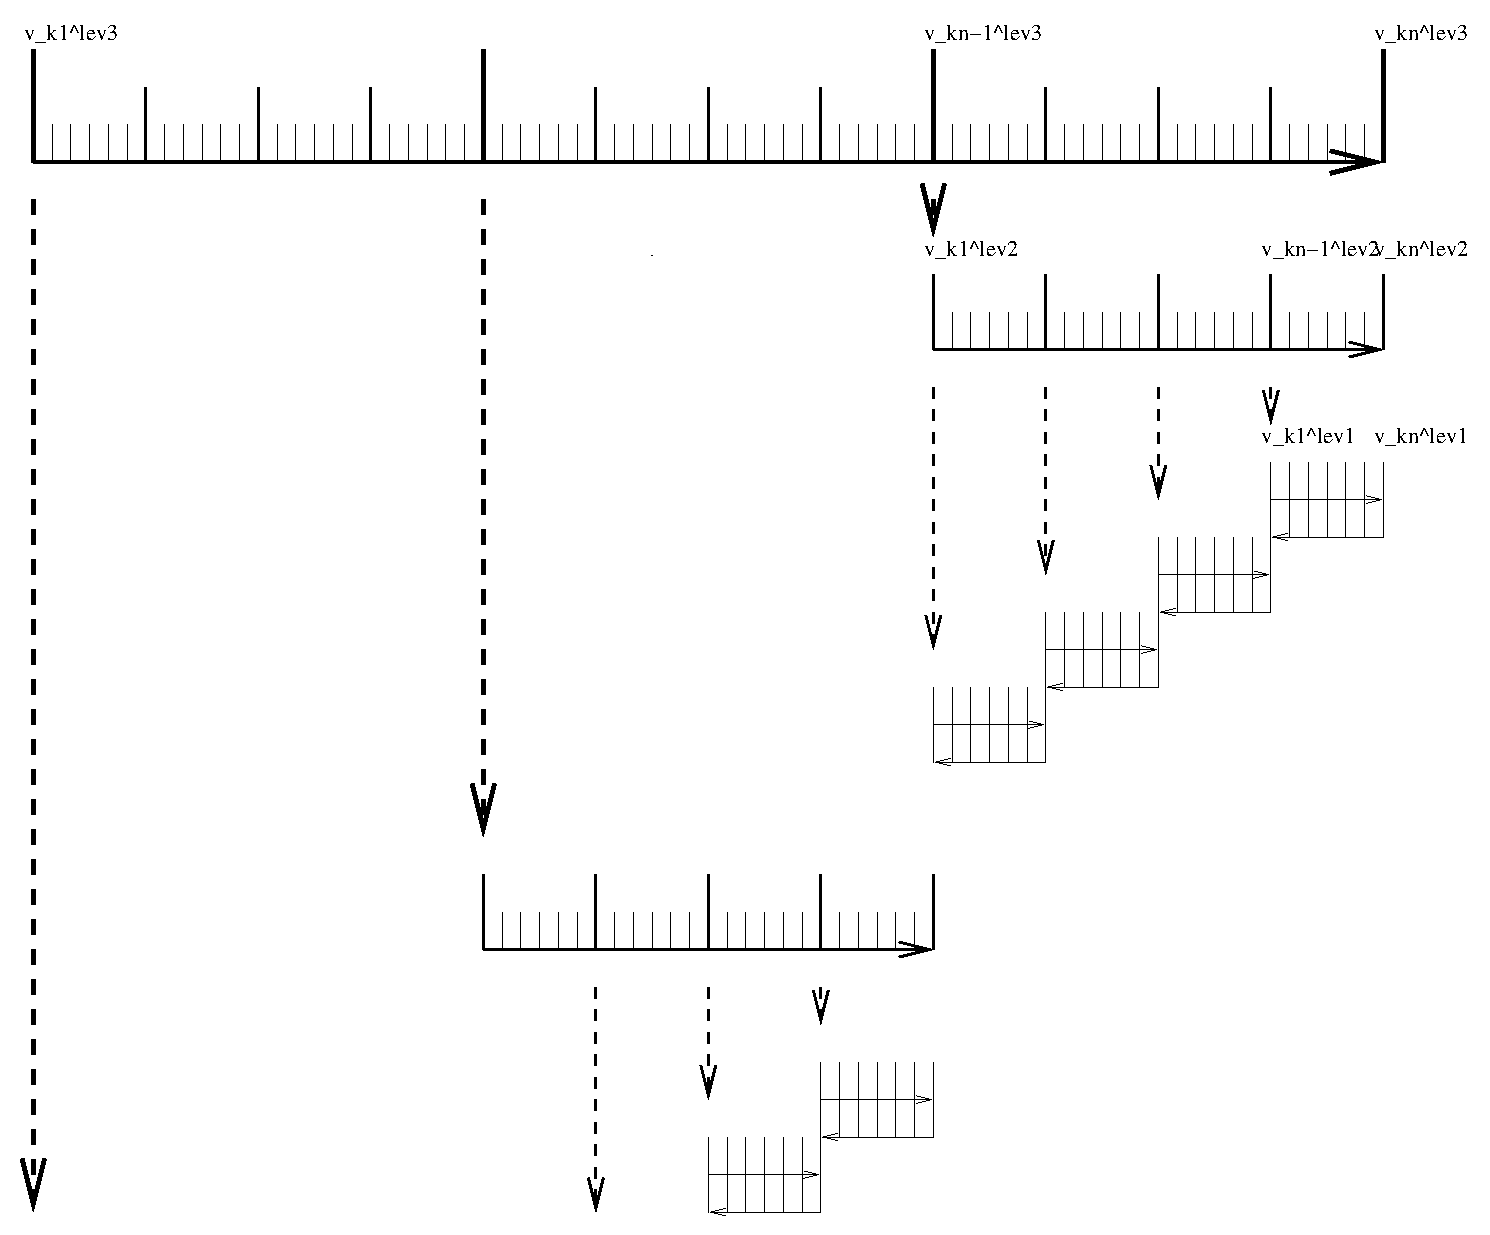
\epsfig{file=part5/checkpointing.eps, width=0.8\textwidth}}
\resizebox{5.5in}{!}{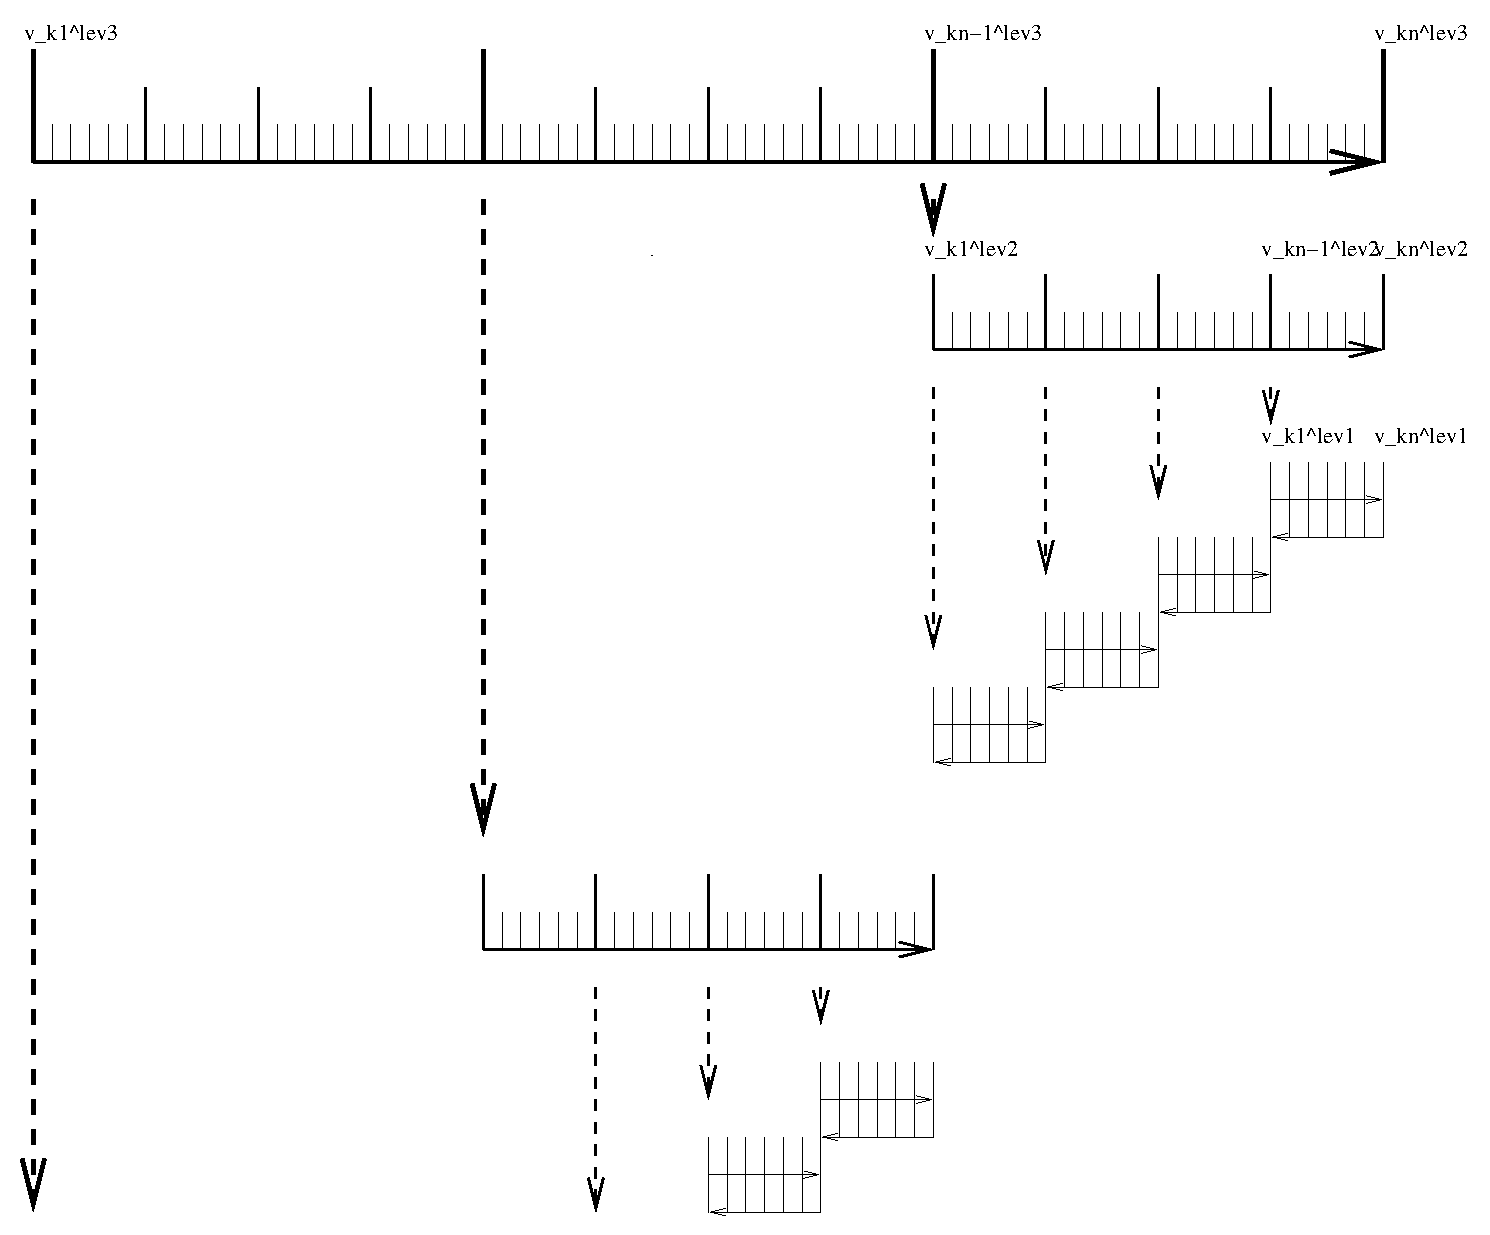
\includegraphics{part5/checkpointing.eps}}
%\psfull
\end{center}
\caption{
Schematic view of intermediate dump and restart for 
3-level checkpointing.}
\label{fig:3levelcheck}
\end{figure}

% \subsection{Optimal perturbations}
% \label{sec_optpert}


% \subsection{Error covariance estimate and Hessian matrix}
% \label{sec_hessian}

\newpage 

%**********************************************************************
\section{TLM and ADM generation in general}
\label{sec_ad_setup_gen}
\begin{rawhtml}
<!-- CMIREDIR:sec_ad_setup_gen: -->
\end{rawhtml}
%**********************************************************************

In this section we describe in a general fashion 
the parts of the code that are relevant for automatic
differentiation using the software tool TAF. 

% $Header: /u/gcmpack/manual/s_autodiff/text/doc_ad_the_model.tex,v 1.3 2001/11/15 15:05:45 cnh Exp $
% $Name:  $
\begin{figure}[b!]

{\scriptsize
\begin{verbatim}
   the_model_main
   |
   |--- initialise_fixed
   |
   |--- #ifdef ALLOW_ADJOINT_RUN
   |           |    
   |           |--- ctrl_unpack
   |           |    
   |           |--- adthe_main_loop
   |           |    |
   |           |    |--- initialise_varia
   |           |    |--- ctrl_map_forcing
   |           |    |--- do iloop = 1, nTimeSteps
   |           |    |       |--- forward_step
   |           |    |       |--- cost_tile
   |           |    |    end do
   |           |    |--- cost_final
   |           |    |
   |           |    |--- adcost_final
   |           |    |--- do iloop = nTimeSteps, 1, -1
   |           |    |       |--- adcost_tile
   |           |    |       |--- adforward_step
   |           |    |    end do
   |           |    |--- adctrl_map_forcing
   |           |    |--- adinitialise_varia
   |           |    o
   |           |
   |           |--- ctrl_pack
   |           |
   |--- #else
   |           |
   |           |--- the_main_loop
   |           |
   |    #endif
   |
   |--- #ifdef ALLOW_GRADIENT_CHECK
   |           |
   |           |--- grdchk_main
   |           o
   |    #endif
   o
\end{verbatim}
}
\caption{~}
\label{fig:adthemodel}
\end{figure}



The basic flow is depicted in \ref{fig:adthemodel}.
If CPP option \texttt{ALLOW\_AUTODIFF\_TAMC} is defined, 
the driver routine
{\it the\_model\_main}, instead of calling {\it the\_main\_loop},
invokes the adjoint of this routine, {\it adthe\_main\_loop}
(case \texttt{\#define ALLOW\_ADJOINT\_RUN}), or
the tangent linear of this routine {\it g\_the\_main\_loop}
(case \texttt{\#define ALLOW\_TANGENTLINEAR\_RUN}),
which are the toplevel routines in terms of automatic differentiation.
The routines {\it adthe\_main\_loop} or {\it g\_the\_main\_loop}
are generated by TAF.
It contains both the forward integration of the full model, the
cost function calculation, 
any additional storing that is required for efficient checkpointing, 
and the reverse integration of the adjoint model.

[DESCRIBE IN A SEPARATE SECTION THE WORKING OF THE TLM]

In Fig. \ref{fig:adthemodel}
the structure of {\it adthe\_main\_loop} has been strongly
simplified to focus on the essentials; in particular, no checkpointing
procedures are shown here.
Prior to the call of {\it adthe\_main\_loop}, the routine
{\it ctrl\_unpack} is invoked to unpack the control vector
or initialise the control variables.
Following the call of {\it adthe\_main\_loop}, 
the routine {\it ctrl\_pack}
is invoked to pack the control vector
(cf. Section \ref{section_ctrl}).
If gradient checks are to be performed, the option 
{\tt ALLOW\_GRADIENT\_CHECK} is defined. In this case
the driver routine {\it grdchk\_main} is called after
the gradient has been computed via the adjoint
(cf. Section \ref{section_grdchk}).

%------------------------------------------------------------------

\subsection{General setup
\label{section_ad_setup}}

In order to configure AD-related setups the following packages need
to be enabled:
{\it
\begin{table}[h!]
\begin{tabular}{l}
autodiff \\
ctrl \\
cost \\
grdchk \\
\end{tabular}
\end{table}
}
The packages are enabled by adding them to your experiment-specific 
configuration file
{\it packages.conf} (see Section ???).

The following AD-specific CPP option files need to be customized:
%
\begin{itemize}
%
\item {\it ECCO\_CPPOPTIONS.h} \\
This header file collects CPP options for the packages
{\it autodiff, cost, ctrl} as well as AD-unrelated options for
the external forcing package {\it exf}.
\footnote{NOTE: These options are not set in their package-specific 
headers such as {\it COST\_CPPOPTIONS.h}, but are instead collected
in the single header file {\it ECCO\_CPPOPTIONS.h}. 
The package-specific header files serve as simple
placeholders at this point.}
%
\item {\it tamc.h} \\
This header configures the splitting of the time stepping loop
w.r.t. the 3-level checkpointing (see section ???).

%
\end{itemize}

%------------------------------------------------------------------

\subsection{Building the AD code
\label{section_ad_build}}

The build process of an AD code is very similar to building
the forward model. However, depending on which AD code one wishes
to generate, and on which AD tool is available (TAF or TAMC),
the following {\tt make} targets are available:

\begin{table}[h!]
{\footnotesize
\begin{tabular}{ccll}
~ & {\it AD-target} & {\it output} & {\it description} \\
\hline
\hline
(1) & {\tt <MODE><TOOL>only} & {\tt <MODE>\_<TOOL>\_output.f}  & 
generates code for $<$MODE$>$ using $<$TOOL$>$ \\
~ & ~ & ~ & no {\tt make} dependencies on {\tt .F .h} \\
~ & ~ & ~ & useful for compiling on remote platforms \\
\hline
(2) & {\tt <MODE><TOOL>} & {\tt <MODE>\_<TOOL>\_output.f}  & 
generates code for $<$MODE$>$ using $<$TOOL$>$ \\
~ & ~ & ~ & includes {\tt make} dependencies on {\tt .F .h} \\
~ & ~ & ~ & i.e. input for $<$TOOL$>$ may be re-generated \\
\hline
(3) & {\tt <MODE>all} & {\tt mitgcmuv\_<MODE>}  & 
generates code for $<$MODE$>$ using $<$TOOL$>$ \\
~ & ~ & ~ & and compiles all code \\
~ & ~ & ~ & (use of TAF is set as default) \\
\hline
\hline
\end{tabular}
}
\end{table}
%
Here, the following placeholders are used
%
\begin{itemize}
%
\item [$<$TOOL$>$]
%
\begin{itemize}
%
\item {\tt TAF}
\item {\tt TAMC}
%
\end{itemize}
%
\item [$<$MODE$>$]
%
\begin{itemize}
%
\item {\tt ad} generates the adjoint model (ADM)
\item {\tt ftl} generates the tangent linear model (TLM)
\item {\tt svd} generates both ADM and TLM for \\
singular value decomposition (SVD) type calculations
%
\end{itemize}
%
\end{itemize}

For example, to generate the adjoint model using TAF after routines ({\tt .F})
or headers ({\tt .h}) have been modified, but without compilation,
type {\tt make adtaf};
or, to generate the tangent linear model using TAMC without
re-generating the input code, type {\tt make ftltamconly}.


A typical full build process to generate the ADM via TAF would
look like follows:
\begin{verbatim}
% mkdir build
% cd build
% ../../../tools/genmake2 -mods=../code_ad
% make depend
% make adall
\end{verbatim}

%------------------------------------------------------------------

\subsection{The AD build process in detail
\label{section_ad_build_detail}}

The {\tt make <MODE>all} target consists of the following procedures:

\begin{enumerate}
%
\item
A header file {\tt AD\_CONFIG.h} is generated which contains a CPP option
on which code ought to be generated. Depending on the {\tt make} target,
the contents is
\begin{itemize}
\item
{\tt \#define ALLOW\_ADJOINT\_RUN}
\item
{\tt \#define ALLOW\_TANGENTLINEAR\_RUN}
\item
{\tt \#define ALLOW\_ECCO\_OPTIMIZATION}
\end{itemize}
%
\item
A single file {\tt <MODE>\_input\_code.f} is concatenated 
consisting of all {\tt .f} files that are part of the list {\bf AD\_FILES} 
and all {\tt .flow} files that are part of the list {\bf AD\_FLOW\_FILES}.
%
\item
The AD tool is invoked with the {\bf <MODE>\_<TOOL>\_FLAGS}.
The default AD tool flags in {\tt genmake2} can be overrwritten by
an {\tt adjoint\_options} file (similar to the platform-specific
{\tt build\_options}, see Section ???.
The AD tool writes the resulting AD code into the file
{\tt <MODE>\_input\_code\_ad.f}
%
\item
A short sed script {\tt adjoint\_sed} is applied to 
{\tt <MODE>\_input\_code\_ad.f}
to reinstate {\bf myThid} into the CALL argument list of active file I/O.
The result is written to file {\tt <MODE>\_<TOOL>\_output.f}.
%
\item
All routines are compiled and an executable is generated
(see Table ???).
%
\end{enumerate}

\subsubsection{The list AD\_FILES and {\tt .list} files}

Not all routines are presented to the AD tool.
Routines typically hidden are diagnostics routines which
do not influence the cost function, but may create 
artificial flow dependencies such as I/O of active variables.

{\tt genmake2} generates a list (or variable) {\bf AD\_FILES}
which contains all routines that are shown to the AD tool.
This list is put together from all files with suffix {\tt .list}
that {\tt genmake2} finds in its search directories.
The list file for the core MITgcm routines is in {\tt model/src/}
is called {\tt model\_ad\_diff.list}.
Note that no wrapper routine is shown to TAF. These are either
not visible at all to the AD code, or hand-written AD code
is available (see next section).

Each package directory contains its package-specific
list file {\tt <PKG>\_ad\_diff.list}. For example,
{\tt pkg/ptracers/} contains the file {\tt ptracers\_ad\_diff.list}.
Thus, enabling a package will automatically extend the
{\bf AD\_FILES} list of {\tt genmake2} to incorporate the
package-specific routines.
Note that you will need to regenerate the {\tt Makefile} if
you enable a package (e.g. by adding it to {\tt packages.conf})
and a {\tt Makefile} already exists.

\subsubsection{The list AD\_FLOW\_FILES and {\tt .flow} files}

TAMC and TAF can evaluate user-specified directives
that start with a specific syntax ({\tt CADJ}, {\tt C\$TAF}, {\tt !\$TAF}).
The main categories of directives are STORE directives and
FLOW directives. Here, we are concerned with flow directives,
store directives are treated elsewhere.

Flow directives enable the AD tool to evaluate how it should treat
routines that are 'hidden' by the user, i.e. routines which are
not contained in the {\bf AD\_FILES} list (see previous section), 
but which are called in part of the code that the AD tool does see.
The flow directive tell the AD tool
%
\begin{itemize}
%
\item which subroutine arguments are input/output
\item which subroutine arguments are active
\item which subroutine arguments are required to compute the cost
\item which subroutine arguments are dependent
%
\end{itemize}
%
The syntax for the flow directives can be found in the
AD tool manuals.

{\tt genmake2} generates a list (or variable) {\bf AD\_FLOW\_FILES}
which contains all files with suffix{\tt .flow} that it finds 
in its search directories.
The flow directives for the core MITgcm routines of
{\tt eesupp/src/} and {\tt model/src/}
reside in {\tt pkg/autodiff/}.
This directory also contains hand-written adjoint code
for the MITgcm WRAPPER (see Section ???).

Flow directives for package-specific routines are contained in
the corresponding package directories in the file
{\tt <PKG>\_ad.flow}, e.g. ptracers-specific directives are in
{\tt ptracers\_ad.flow}.

\subsubsection{Store directives for 3-level checkpointing}

The storing that is required at each period of the
3-level checkpointing is controled by three
top-level headers.

\begin{verbatim}
do ilev_3 = 1, nchklev_3
#  include ``checkpoint_lev3.h''
   do ilev_2 = 1, nchklev_2
#     include ``checkpoint_lev2.h''
      do ilev_1 = 1, nchklev_1
#        include ``checkpoint_lev1.h''

...

      end do
   end do
end do
\end{verbatim}

All files {\tt checkpoint\_lev?.h} are contained in directory
{\tt pkg/autodiff/}.


\subsubsection{Changing the default AD tool flags: ad\_options files}


\subsubsection{Hand-written adjoint code}

%------------------------------------------------------------------

\subsection{The cost function (dependent variable)
\label{section_cost}}

The cost function $ {\cal J} $ is referred to as the {\sf dependent variable}.
It is a function of the input variables $ \vec{u} $ via the composition
$ {\cal J}(\vec{u}) \, = \, {\cal J}(M(\vec{u})) $. 
The input are referred to as the
{\sf independent variables} or {\sf control variables}.
All aspects relevant to the treatment of the cost function $ {\cal J} $
(parameter setting, initialization, accumulation, 
final evaluation), are controlled by the package {\it pkg/cost}.
The aspects relevant to the treatment of the independent variables
are controlled by the package {\it pkg/ctrl} and will be treated
in the next section.

\begin{figure}[!ht]

{\scriptsize
\begin{verbatim}
      the_model_main
      |
      |-- initialise_fixed
      |   |
      |   |-- packages_readparms
      |       |
      |       |-- cost_readparms
      |       o
      |
      |-- the_main_loop
     ...  |
          |-- initialise_varia
          |   |
          |   |-- packages_init_variables
          |       |
          |       |-- cost_init
          |       o
          |
          |-- do iloop = 1,nTimeSteps
          |      |-- forward_step
          |      |-- cost_tile
          |      |   |
          |      |   |-- cost_tracer
          |   end do
          |
          |-- cost_final
          o
\end{verbatim}
}

\caption{~}
\label{fig:costflow}
\end{figure}


\subsubsection{Enabling the package}

\fbox{
\begin{minipage}{12cm}
{\it packages.conf}, {\it ECCO\_CPPOPTIONS.h}
\end{minipage}
}
\begin{itemize}
%
\item
The package is enabled by adding {\it cost} to your file {\it packages.conf}
(see Section ???)
%
\item


\end{itemize}
%

N.B.: In general the following packages ought to be enabled
simultaneously: {\it autodiff, cost, ctrl}.
The basic CPP option to enable the cost function is {\bf ALLOW\_COST}.
Each specific cost function contribution has its own option.
For the present example the option is {\bf ALLOW\_COST\_TRACER}.
All cost-specific options are set in {\it ECCO\_CPPOPTIONS.h}
Since the cost function is usually used in conjunction with
automatic differentiation, the CPP option
{\bf ALLOW\_ADJOINT\_RUN} (file {\it CPP\_OPTIONS.h}) and
{\bf ALLOW\_AUTODIFF\_TAMC} (file {\it ECCO\_CPPOPTIONS.h})
should be defined.

\subsubsection{Initialization}
%
The initialization of the {\it cost} package is readily enabled
as soon as the CPP option {\bf ALLOW\_COST} is defined.
%
\begin{itemize}
%
\item 
\fbox{
\begin{minipage}{12cm}
Parameters: {\it cost\_readparms}
\end{minipage}
}
\\
This S/R 
reads runtime flags and parameters from file {\it data.cost}.
For the present example the only relevant parameter read
is {\bf mult\_tracer}. This multiplier enables different
cost function contributions to be switched on
( = 1.) or off ( = 0.) at runtime.
For more complex cost functions which involve model vs. data
misfits, the corresponding data filenames and data
specifications (start date and time, period, ...) are read
in this S/R.
%
\item 
\fbox{
\begin{minipage}{12cm}
Variables: {\it cost\_init}
\end{minipage}
}
\\
This S/R 
initializes the different cost function contributions.
The contribution for the present example is {\bf objf\_tracer}
which is defined on each tile (bi,bj).
%
\end{itemize}
%
\subsubsection{Accumulation}
%
\begin{itemize}
%
\item 
\fbox{
\begin{minipage}{12cm}
{\it cost\_tile}, {\it cost\_tracer}
\end{minipage}
}
\end{itemize}
%
The 'driver' routine
{\it cost\_tile} is called at the end of each time step.
Within this 'driver' routine, S/R are called for each of
the chosen cost function contributions.
In the present example ({\bf ALLOW\_COST\_TRACER}),
S/R {\it cost\_tracer} is called.
It accumulates {\bf objf\_tracer} according to eqn. (\ref{???}).
%
\subsubsection{Finalize all contributions}
%
\begin{itemize}
%
\item 
\fbox{
\begin{minipage}{12cm}
{\it cost\_final}
\end{minipage}
}
\end{itemize}
%
At the end of the forward integration S/R {\it cost\_final}
is called. It accumulates the total cost function {\bf fc}
from each contribution and sums over all tiles:
\begin{equation}
{\cal J} \, = \, 
{\rm fc} \, = \, 
{\rm mult\_tracer} \sum_{\text{global sum}} \sum_{bi,\,bj}^{nSx,\,nSy}
{\rm objf\_tracer}(bi,bj) \, + \, ...
\end{equation}
%
The total cost function {\bf fc} will be the
'dependent' variable in the argument list for TAMC, i.e.
\begin{verbatim}
tamc -output 'fc' ...
\end{verbatim}

%%%% \end{document}

% $Header: /u/gcmpack/manual/s_autodiff/text/doc_ad_the_main.tex,v 1.3 2001/11/15 16:57:48 cnh Exp $
% $Name:  $
\begin{figure}

{\scriptsize
\begin{verbatim}
   *************
   the_main_loop
   *************
   |
   |--- initialise_varia
   |    |
   |   ...
   |    |--- packages_init_varia
   |    |    |
   |    |   ...
   |    |    |--- #ifdef ALLOW_ADJOINT_RUN
   |    |    |          call ctrl_map_ini
   |    |    |          call cost_ini
   |    |    |    #endif
   |    |   ...
   |    |    o
   |   ...
   |    o
  ...
   |--- #ifdef ALLOW_ADJOINT_RUN
   |          call ctrl_map_forcing
   |    #endif
  ...
   |--- #ifdef ALLOW_TAMC_CHECKPOINTING
              do ilev_3 = 1,nchklev_3
   |            do ilev_2 = 1,nchklev_2
   |              do ilev_1 = 1,nchklev_1
   |                iloop = (ilev_3-1)*nchklev_2*nchklev_1 +
   |                        (ilev_2-1)*nchklev_1           + ilev_1
   |    #else
   |          do iloop = 1, nTimeSteps
   |    #endif
   |    |
   |    |---       call forward_step
   |    |
   |    |--- #ifdef ALLOW_COST
   |    |          call cost_tile
   |    |    #endif
   |    |
   |    |    enddo
   |    o
   |
   |--- #ifdef ALLOW_COST
   |          call cost_final
   |    #endif
   o
\end{verbatim}
}
\caption{~}
\label{fig:adthemain}
\end{figure}


\subsection{The control variables (independent variables)
\label{section_ctrl}}

The control variables are a subset of the model input
(initial conditions, boundary conditions, model parameters).
Here we identify them with the variable $ \vec{u} $.
All intermediate variables whose derivative w.r.t. control
variables do not vanish are called {\sf active variables}.
All subroutines whose derivative w.r.t. the control variables
don't vanish are called {\sf active routines}.
Read and write operations from and to file can be viewed
as variable assignments. Therefore, files to which
active variables are written and from which active variables
are read are called {\sf active files}.
All aspects relevant to the treatment of the control variables
(parameter setting, initialization, perturbation)
are controlled by the package {\it pkg/ctrl}.

\begin{figure}[h!]

{\scriptsize
\begin{verbatim}
          the_model_main
          |
          |-- initialise_fixed
          |   |
          |   |-- packages_readparms
          |       |
          |       |-- ctrl_init                - initialise control
          |       o                              package
          |
          |-- ctrl_unpack                      - unpack control vector
          |
          |-- adthe_main_loop                  - forward/adjoint run
          |   |
          |   |-- initialise_variables
          |   |   |
          |   |   |-- packages_init_variables
          |   |       |
          |   |       |-- ctrl_map_ini         - link init. state and
          |   |       o                          parameters to control 
          |   |                                  variables
          |   |-- ctrl_map_forcing             - link forcing fields to
          |  ...                                 control variables
          |
          |-- ctrl_pack                        - pack control vector
\end{verbatim}
}
\caption{~}
\label{fig:ctrlflow}
\end{figure}


\subsubsection{genmake and CPP options}
%
\begin{itemize}
%
\item 
\fbox{
\begin{minipage}{12cm}
{\it genmake}, {\it CPP\_OPTIONS.h}, {\it ECCO\_CPPOPTIONS.h}
\end{minipage}
}
\end{itemize}
%
To enable the directory to be included to the compile list,
{\bf ctrl} has to be added to the {\bf enable} list in
{\it .genmakerc} or in {\it genmake} itself (analogous to {\it cost}
package, cf. previous section).
Each control variable is enabled via its own CPP option
in {\it ECCO\_CPPOPTIONS.h}.

\subsubsection{Initialization}
%
\begin{itemize}
%
\item 
\fbox{
\begin{minipage}{12cm}
Parameters: {\it ctrl\_readparms}
\end{minipage}
}
\\
%
This S/R 
reads runtime flags and parameters from file {\it data.ctrl}.
For the present example the file contains the file names
of each control variable that is used.
In addition, the number of wet points for each control
variable and the net dimension of the space of control
variables (counting wet points only) {\bf nvarlength}
is determined.
Masks for wet points for each tile {\bf (bi,\,bj)}
and vertical layer {\bf k} are generated for the three
relevant categories on the C-grid:
{\bf nWetCtile} for tracer fields, 
{\bf nWetWtile} for zonal velocity fields,
{\bf nWetStile} for meridional velocity fields.
%
\item 
\fbox{
\begin{minipage}{12cm}
Control variables, control vector,
and their gradients: {\it ctrl\_unpack}
\end{minipage}
}
\\
%
Two important issues related to the handling of the control
variables in the MITGCM need to be addressed.
First, in order to save memory, the control variable arrays
are not kept in memory, but rather read from file and added
to the initial fields during the model initialization phase.
Similarly, the corresponding adjoint fields which represent
the gradient of the cost function w.r.t. the control variables
are written to file at the end of the adjoint integration.
Second, in addition to the files holding the 2-dim. and 3-dim.
control variables and the corresponding cost gradients, 
a 1-dim. {\sf control vector} 
and {\sf gradient vector} are written to file. They contain 
only the wet points of the control variables and the corresponding 
gradient.
This leads to a significant data compression.
Furthermore, an option is available
({\tt ALLOW\_NONDIMENSIONAL\_CONTROL\_IO}) to
non-dimensionalise the control and gradient vector,
which otherwise would contain different pieces of different
magnitudes and units.
Finally, the control and gradient vector can be passed to a 
minimization routine if an update of the control variables
is sought as part of a minimization exercise.

The files holding fields and vectors of the control variables
and gradient are generated and initialised in S/R {\it ctrl\_unpack}.
%
\end{itemize}

\subsubsection{Perturbation of the independent variables}
%
The dependency flow for differentiation w.r.t. the controls 
starts with adding a perturbation onto the input variable,
thus defining the independent or control variables for TAMC.
Three types of controls may be considered:
%
\begin{itemize}
%
\item 
\fbox{
\begin{minipage}{12cm}
{\it ctrl\_map\_ini} (initial value sensitivity): 
\end{minipage}
}
\\
%
Consider as an example the initial tracer distribution
{\bf tr1} as control variable.
After {\bf tr1} has been initialised in
{\it ini\_tr1} (dynamical variables such as
temperature and salinity are initialised in {\it ini\_fields}),
a perturbation anomaly is added to the field in S/R
{\it ctrl\_map\_ini}
%
\begin{equation}
\begin{split}
u         & = \, u_{[0]} \, + \, \Delta u \\
{\bf tr1}(...) & = \, {\bf tr1_{ini}}(...) \, + \, {\bf xx\_tr1}(...)
\label{perturb}
\end{split}
\end{equation}
%
{\bf xx\_tr1} is a 3-dim. global array 
holding the perturbation. In the case of a simple
sensitivity study this array is identical to zero.
However, it's specification is essential in the context
of automatic differentiation since TAMC
treats the corresponding line in the code symbolically
when determining the differentiation chain and its origin.
Thus, the variable names are part of the argument list
when calling TAMC: 
%
\begin{verbatim}
tamc -input 'xx_tr1 ...' ...
\end{verbatim}
%
Now, as mentioned above, the MITGCM avoids maintaining
an array for each control variable by reading the
perturbation to a temporary array from file.
To ensure the symbolic link to be recognized by TAMC, a scalar
dummy variable {\bf xx\_tr1\_dummy} is introduced
and an 'active read' routine of the adjoint support
package {\it pkg/autodiff} is invoked.
The read-procedure is tagged with the variable
{\bf xx\_tr1\_dummy} enabling TAMC to recognize the
initialization of the perturbation.
The modified call of TAMC thus reads
%
\begin{verbatim}
tamc -input 'xx_tr1_dummy ...' ...
\end{verbatim}
%
and the modified operation to (\ref{perturb})
in the code takes on the form
%
\begin{verbatim}
       call active_read_xyz( 
     &      ..., tmpfld3d, ..., xx_tr1_dummy, ... )

       tr1(...) = tr1(...) + tmpfld3d(...)
\end{verbatim}
%
Note, that reading an active variable corresponds
to a variable assignment. Its derivative corresponds
to a write statement of the adjoint variable, followed by
a reset.
The 'active file' routines have been designed
to support active read and corresponding adjoint active write
operations (and vice versa).
%
\item 
\fbox{
\begin{minipage}{12cm}
{\it ctrl\_map\_forcing} (boundary value sensitivity): 
\end{minipage}
}
\\
%
The handling of boundary values as control variables
proceeds exactly analogous to the initial values
with the symbolic perturbation taking place in S/R
{\it ctrl\_map\_forcing}.
Note however an important difference:
Since the boundary values are time dependent with a new
forcing field applied at each time steps,
the general problem may be thought of as
a new control variable at each time step
(or, if the perturbation is averaged over a certain period,
at each $ N $ timesteps), i.e.
\[
u_{\rm forcing} \, = \,
\{ \, u_{\rm forcing} ( t_n ) \, \}_{
n \, = \, 1, \ldots , {\rm nTimeSteps} }
\]
%
In the current example an equilibrium state is considered,
and only an initial perturbation to
surface forcing is applied with respect to the
equilibrium state.
A time dependent treatment of the surface forcing is 
implemented in the ECCO environment, involving the
calendar ({\it cal}~) and external forcing ({\it exf}~) packages.
%
\item 
\fbox{
\begin{minipage}{12cm}
{\it ctrl\_map\_params} (parameter sensitivity): 
\end{minipage}
}
\\
%
This routine is not yet implemented, but would proceed
proceed along the same lines as the initial value sensitivity.
The mixing parameters {\bf diffkr} and {\bf kapgm}
are currently added as controls in {\it ctrl\_map\_ini.F}.
%
\end{itemize}
%

\subsubsection{Output of adjoint variables and gradient}
%
Several ways exist to generate output of adjoint fields.
%
\begin{itemize}
%
\item 
\fbox{
\begin{minipage}{12cm}
{\it ctrl\_map\_ini, ctrl\_map\_forcing}: 
\end{minipage}
}
\\
\begin{itemize}
%
\item {\bf xx\_...}: the control variable fields \\
Before the forward integration, the control
variables are read from file {\bf xx\_ ...} and added to
the model field.
%
\item {\bf adxx\_...}: the adjoint variable fields, i.e. the gradient
$ \nabla _{u}{\cal J} $ for each control variable \\
After the adjoint integration the corresponding adjoint
variables are written to {\bf adxx\_ ...}.
%
\end{itemize}
%
\item 
\fbox{
\begin{minipage}{12cm}
{\it ctrl\_unpack, ctrl\_pack}: 
\end{minipage}
}
\\
%
\begin{itemize}
%
\item {\bf vector\_ctrl}: the control vector \\
At the very beginning of the model initialization,
the updated compressed control vector is read (or initialised)
and distributed to 2-dim. and 3-dim. control variable fields.
%
\item {\bf vector\_grad}: the gradient vector \\
At the very end of the adjoint integration,
the 2-dim. and 3-dim. adjoint variables are read,
compressed to a single vector and written to file.
%
\end{itemize}
%
\item 
\fbox{
\begin{minipage}{12cm}
{\it addummy\_in\_stepping}: 
\end{minipage}
}
\\
In addition to writing the gradient at the end of the
forward/adjoint integration, many more adjoint variables
of the model state
at intermediate times can be written using S/R 
{\it addummy\_in\_stepping}.
This routine is part of the adjoint support package 
{\it pkg/autodiff} (cf.f. below).
The procedure is enabled using via the CPP-option
{\bf ALLOW\_AUTODIFF\_MONITOR} (file {\it ECCO\_CPPOPTIONS.h}).
To be part of the adjoint code, the corresponding S/R
{\it dummy\_in\_stepping} has to be called in the forward
model (S/R {\it the\_main\_loop}) at the appropriate place.
The adjoint common blocks are extracted from the adjoint code
via the header file {\it adcommon.h}.

{\it dummy\_in\_stepping} is essentially empty,
the corresponding adjoint routine is hand-written rather
than generated automatically.
Appropriate flow directives ({\it dummy\_in\_stepping.flow})
ensure that TAMC does not automatically 
generate {\it addummy\_in\_stepping} by trying to differentiate
{\it dummy\_in\_stepping}, but instead refers to 
the hand-written routine.

{\it dummy\_in\_stepping} is called in the forward code
at the beginning of each
timestep, before the call to {\it dynamics}, thus ensuring
that {\it addummy\_in\_stepping} is called at the end of
each timestep in the adjoint calculation, after the call to
{\it addynamics}.

{\it addummy\_in\_stepping} includes the header files
{\it adcommon.h}.
This header file is also hand-written. It contains
the common blocks 
{\bf /addynvars\_r/}, {\bf /addynvars\_cd/},
{\bf /addynvars\_diffkr/}, {\bf /addynvars\_kapgm/},
{\bf /adtr1\_r/}, {\bf /adffields/},
which have been extracted from the adjoint code to enable
access to the adjoint variables.

{\bf WARNING:} If the structure of the common blocks
{\bf /dynvars\_r/}, {\bf /dynvars\_cd/}, etc., changes
similar changes will occur in the adjoint common blocks.
Therefore, consistency between the TAMC-generated common blocks
and those in {\it adcommon.h} have to be checked.
%
\end{itemize}


\subsubsection{Control variable handling for 
optimization applications}

In optimization mode the cost function $ {\cal J}(u) $ is sought
to be minimized with respect to a set of control variables
$ \delta {\cal J} \, = \, 0 $, in an iterative manner.
The gradient $ \nabla _{u}{\cal J} |_{u_{[k]}} $ together
with the value of the cost function itself $ {\cal J}(u_{[k]}) $ 
at iteration step $ k $ serve
as input to a minimization routine (e.g. quasi-Newton method,
conjugate gradient, ... \cite{gil-lem:89}) 
to compute an update in the
control variable for iteration step $k+1$
\[
u_{[k+1]} \, = \,  u_{[0]} \, + \, \Delta u_{[k+1]}
\quad \mbox{satisfying} \quad
 {\cal J} \left( u_{[k+1]} \right) \, < \, {\cal J} \left( u_{[k]} \right)
\]
$ u_{[k+1]} $ then serves as input for a forward/adjoint run
to determine $ {\cal J} $ and $ \nabla _{u}{\cal J} $ at iteration step
$ k+1 $.
Tab. \ref{???} sketches the flow between forward/adjoint model
and the minimization routine.

\begin{eqnarray*}
\scriptsize
\begin{array}{ccccc}
u_{[0]} \,\, ,  \,\, \Delta u_{[k]}    & ~ & ~ & ~ & ~ \\
{\Big\downarrow} 
   & ~ & ~ & ~ & ~ \\
 ~ & ~ & ~ & ~ & ~ \\
\hline
\multicolumn{1}{|c}{~} & ~ & ~ & ~ & \multicolumn{1}{c|}{~} \\
\multicolumn{1}{|c}{
u_{[k]} = u_{[0]} + \Delta u_{[k]}} &
\stackrel{\bf forward}{\bf \longrightarrow} &
v_{[k]} = M \left( u_{[k]} \right) &
\stackrel{\bf forward}{\bf \longrightarrow} &
\multicolumn{1}{c|}{
{\cal J}_{[k]} = {\cal J} \left( M \left( u_{[k]} \right) \right)} \\
\multicolumn{1}{|c}{~} & ~ & ~ & ~ & \multicolumn{1}{c|}{~} \\
\hline
\multicolumn{1}{|c}{~} & ~ & ~ & ~ & \multicolumn{1}{c|}{~}  \\
\multicolumn{1}{|c}{~} & ~ & ~ & ~ & \multicolumn{1}{c|}{{\Big\downarrow}} \\
\multicolumn{1}{|c}{~} & ~ & ~ & ~ & \multicolumn{1}{c|}{~}  \\
\hline
\multicolumn{1}{|c}{~} & ~ & ~ & ~ & \multicolumn{1}{c|}{~} \\
\multicolumn{1}{|c}{
\nabla_u {\cal J}_{[k]} (\delta {\cal J}) = 
T^{\ast} \cdot \nabla_v {\cal J} |_{v_{[k]}} (\delta {\cal J})} &
\stackrel{\bf adjoint}{\mathbf \longleftarrow} &
ad \, v_{[k]} (\delta {\cal J}) = 
\nabla_v {\cal J} |_{v_{[k]}} (\delta {\cal J}) &
\stackrel{\bf adjoint}{\mathbf \longleftarrow} &
\multicolumn{1}{c|}{ ad \, {\cal J} = \delta {\cal J}} \\
\multicolumn{1}{|c}{~} & ~ & ~ & ~ & \multicolumn{1}{c|}{~} \\
\hline
 ~ & ~ & ~ & ~ & ~ \\
\hspace*{15ex}{\Bigg\downarrow}  
\quad {\cal J}_{[k]}, \quad \nabla_u {\cal J}_{[k]}
 & ~ & ~ & ~ & ~ \\
 ~ & ~ & ~ & ~ & ~ \\
\hline
\multicolumn{1}{|c}{~} & ~ & ~ & ~ & \multicolumn{1}{c|}{~} \\
\multicolumn{1}{|c}{
{\cal J}_{[k]} \,\, ,  \,\, \nabla_u {\cal J}_{[k]}} &
{\mathbf \longrightarrow} & \text{\bf minimisation} &
{\mathbf \longrightarrow} & 
\multicolumn{1}{c|}{ \Delta u_{[k+1]}} \\
\multicolumn{1}{|c}{~} & ~ & ~ & ~ & \multicolumn{1}{c|}{~} \\
\hline
 ~ & ~ & ~ & ~ & ~ \\
 ~ & ~ & ~ & ~ & \Big\downarrow \\
 ~ & ~ & ~ & ~ & \Delta u_{[k+1]} \\
\end{array}
\end{eqnarray*}

The routines {\it ctrl\_unpack} and {\it ctrl\_pack} provide
the link between the model and the minimization routine.
As described in Section \ref{???} 
the {\it unpack} and {\it pack} routines read and write
control and gradient {\it vectors} which are compressed
to contain only wet points, in addition to the full
2-dim. and 3-dim. fields. 
The corresponding I/O flow looks as follows:

\vspace*{0.5cm}

{\scriptsize
\begin{tabular}{ccccc}
{\bf vector\_ctrl\_$<$k$>$ } & ~ & ~ & ~ & ~ \\
{\big\downarrow}  & ~ & ~ & ~ & ~ \\
\cline{1-1}
\multicolumn{1}{|c|}{\it ctrl\_unpack} & ~ & ~ & ~ & ~ \\
\cline{1-1}
{\big\downarrow}  & ~ & ~ & ~ & ~ \\
\cline{3-3}
\multicolumn{1}{l}{\bf xx\_theta0...$<$k$>$} & ~ &
\multicolumn{1}{|c|}{~} & ~ & ~ \\
\multicolumn{1}{l}{\bf xx\_salt0...$<$k$>$} & 
$\stackrel{\mbox{read}}{\longrightarrow}$ &
\multicolumn{1}{|c|}{forward integration} & ~ & ~ \\ 
\multicolumn{1}{l}{\bf \vdots} & ~ & \multicolumn{1}{|c|}{~}  
& ~ & ~ \\
\cline{3-3}
~ & ~ & $\downarrow$ & ~ & ~ \\
\cline{3-3}
~ & ~ & 
\multicolumn{1}{|c|}{~} & ~ & 
\multicolumn{1}{l}{\bf adxx\_theta0...$<$k$>$}  \\
~ & ~ & \multicolumn{1}{|c|}{adjoint integration} & 
$\stackrel{\mbox{write}}{\longrightarrow}$ & 
\multicolumn{1}{l}{\bf adxx\_salt0...$<$k$>$} \\ 
~ & ~ & \multicolumn{1}{|c|}{~}  
& ~ & \multicolumn{1}{l}{\bf \vdots} \\
\cline{3-3}
~ & ~ & ~ & ~ & {\big\downarrow} \\
\cline{5-5}
~ & ~ & ~ & ~ & \multicolumn{1}{|c|}{\it ctrl\_pack} \\
\cline{5-5}
~ & ~ & ~ & ~ &  {\big\downarrow} \\
~ & ~ & ~ & ~ &  {\bf vector\_grad\_$<$k$>$ } \\
\end{tabular}
}

\vspace*{0.5cm}


{\it ctrl\_unpack} reads the updated control vector
{\bf vector\_ctrl\_$<$k$>$}.
It distributes the different control variables to
2-dim. and 3-dim. files {\it xx\_...$<$k$>$}.
At the start of the forward integration the control variables
are read from {\it xx\_...$<$k$>$} and added to the
field.
Correspondingly, at the end of the adjoint integration
the adjoint fields are written
to {\it adxx\_...$<$k$>$}, again via the active file routines.
Finally, {\it ctrl\_pack} collects all adjoint files
and writes them to the compressed vector file
{\bf vector\_grad\_$<$k$>$}.
